\subsection{Innovation}

Grundsätzlich bietet das System kurz und mittelfristige Lagerung von Fahrrädern zu einem geringen Nutzpreis an. Dies passiert auf geringstem Raum, gewährleistet jedoch Sicherheit vor Diebstahl im Gegensatz zu herkömmlichen Fahrradständern. Nutzer können ihr Fahrrad mit einer App ganz einfach lagern und abholen, zudem kann man in der App Infos zu nahegelegenen Türmen erhalten.


Es gibt schon einige andere Firmen, die automatische Fahrradparksysteme anbieten, bis jetzt hat sich jedoch kein Konkurrent als Markführer gezeigt. Das System lernt aus den Fehlern bestehender, unerfolgreicher Fahrradlagertürme und hebt sich mit einigen grundlegenden Features von der Konkurrenz ab.


Die vom Projektteam entworfenen Fahrradtürme sind mobil und modular, das bedeutet, dass die Türme aus einzelnen Segmenten bestehen, die je nach Bedarf an verschiedenen Orten auf- und abgebaut werden können. Bei einem großen Event, könnte so zum Beispiel ein Turm temporär aufgestellt werden, um der erhöhten Nachfrage nachzukommen.


Im Gegensatz zu Konkurrenten limitiert sich das System nicht ausschließlich auf Fahrräder, denn andere muskel- und E-motorgetriebene Kleinfahrzeuge werden immer häufiger. Der Turm ist so konzipiert, dass alle möglichen Fahrzeuge - und Gegenstände - gelagert werden können. So verbreitert das Projektteam das Einsatzspektrum und erhöht zugleich die Anzahl potenzieller Kunden. Auch Pakete können in vorgesehenen Plätzen kurzfristig gelagert werden. Das ermöglicht Kooperationen mit etwaigen Versandunternehmen, sodass ein Paket einfach vom Lieferanten zu deinem Fahrrad gelegt werden kann.

\begin{figure}[H]
  \centering
  \begin{subfigure}{0.4\textwidth}
    \centering
    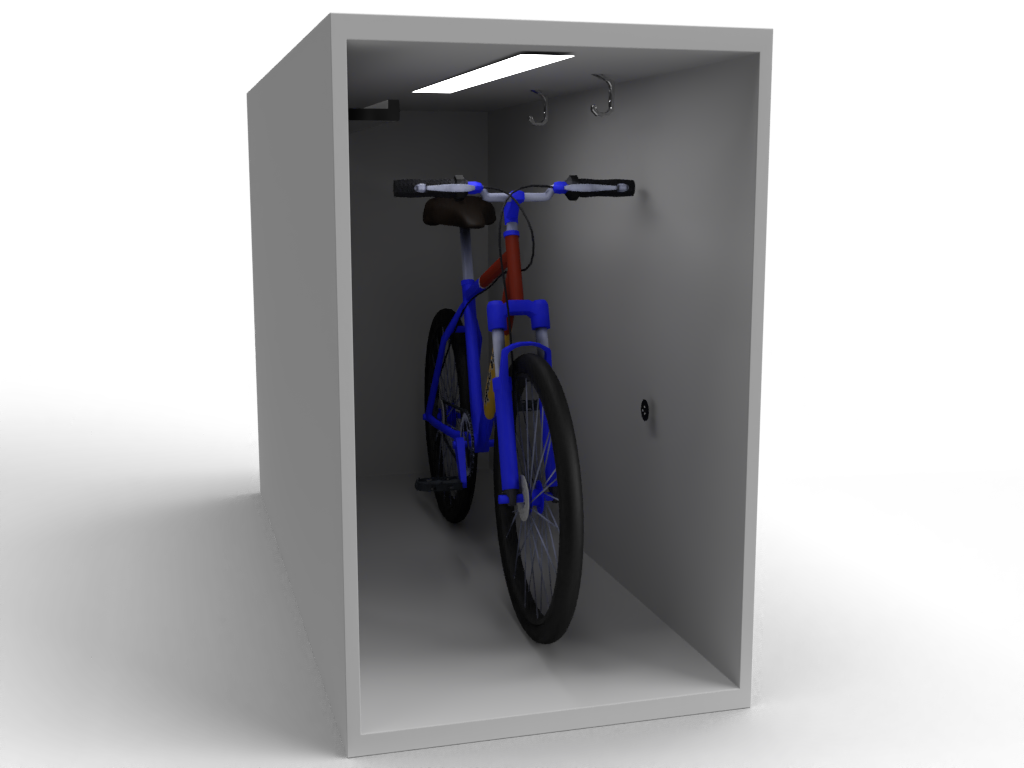
\includegraphics[width=\textwidth]{images/box_bike.png}
    \caption{Lagerung eines Fahrrads}
    \label{fig:storing_bike}
  \end{subfigure}
  \begin{subfigure}{0.4\textwidth}
    \centering
    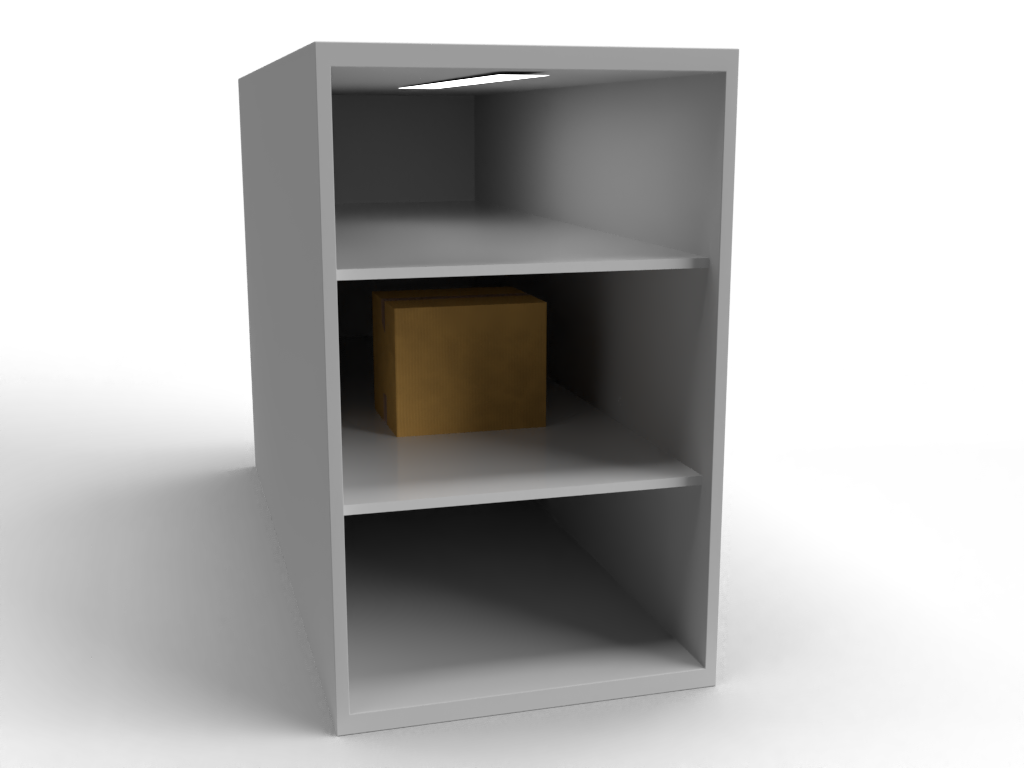
\includegraphics[width=\textwidth]{images/box_item.png}
    \caption{Lagerung eines Pakets}
    \label{fig:storing_item}
  \end{subfigure}
\end{figure}

Mit der App kann man nicht nur ein Paket erhalten, sondern auch viele andere Möglichkeiten bieten sich an. Man ist zum Beispiel auf dem Weg ins Büro und sein Fahrradschlauch platzt. Mit der App kann ganz einfach ein Fahrradservice beantragt werden und nach der Arbeit hat man ein frisch Repariertes Fahrrad. Leihfahrrad und -Scooter Dienste sollen bei Bedarf auch ihre Fahrzeuge im Turm zwischenlagern lassen, um Beschädigung und Unordnung auf der Straße zu vermeiden. E-Scooter dürfen in Wien ab Mai 2023 zum Beispiel nicht mehr auf dem Gehsteig abgestellt werden\cite{krutzler_wien_2022}.